%**************************************************************************
%*                      Team 27 - SimCLR on STL-10                       *
%*         ELECTRONIC LETTERS ON COMPUTER VISION AND IMAGE ANALYSIS       *
%*                      LaTex 2e Document                                 *
%**************************************************************************

\documentclass[twoside,a4paper,11pt]{article}
\usepackage{times}
\usepackage{elcvia}
\usepackage[english]{babel}
\usepackage{graphicx}
\usepackage{amsmath}
\usepackage{booktabs}
\usepackage{url}
\usepackage{float}
\usepackage{enumitem}

% INFORMATION TO FILL IN CAMERA READY VERSION
%------------------------------------------------------------------
\newcommand{\vol}{0}
\newcommand{\num}{0}
\setcounter{page}{1}
\newcommand{\begpag}{\thepage}
\newcommand{\finpag}{10}
\newcommand{\yearp}{2026}
%------------------------------------------------------------------
\renewcommand{\thefootnote}{\fnsymbol{footnote}}

\title{Self-supervised Contrastive Pretraining When Labels Are Scarce:
SimCLR on STL-10
\footnote[0]{Correspondence to: nidhi@university.edu \vspace{0.2cm}}
\footnote[0]{\noindent Recommended for acceptance by $<$name$>$}
\footnote[0]{ELCVIA ISSN:1577-5097}
\footnote[0]{Published by Computer Vision Center / Universitat Aut\`onoma de
Barcelona, Barcelona, Spain}
}

\author{Shubham Kang$^*$, Sandhya Parmar$^+$ and Nidhi Kumari$^\dagger$ \\ \\
\centerline{\small \em $^*$ Department of Computer Science, University, City, Country} \\
\centerline{\small \em $^+$ Department of Computer Science, University, City, Country} \\
\centerline{\small \em $^\dagger$ Department of Computer Science, University, City, Country} \\ \\
\centerline{\small Received 1 January 2026; revised 1 January 2026; accepted 1 January 2026}
}

\begin{document}

\maketitle

\pagestyle{myheadings}
\markboth{\centerline{\small \it Kang et al. /
           Electronic Letters on Computer Vision and Image Analysis
           \vol(\num):\begpag-\finpag, \yearp}}
         {\centerline{\small \it Kang et al. /
           Electronic Letters on Computer Vision and Image Analysis
           \vol(\num):\begpag-\finpag, \yearp}}
\hrulefill

% ================================================================
\begin{abstract}

We study SimCLR~\cite{chen2020simclr}, a self-supervised contrastive learning
framework, on the STL-10 benchmark under a small compute budget. Using 100,000
unlabelled images for pretraining and varying the fraction of labels available for
downstream classification (100\%, 20\%, 10\%, 1\%), we show that SimCLR features
substantially outperform a supervised ResNet-18 baseline in the low-label regime. We
further run two ablation studies: a leave-one-out augmentation ablation across five
augmentations (random crop, horizontal flip, colour jitter, grayscale, Gaussian blur),
and a batch-size ablation across four batch sizes (64, 128, 256, 512). Random cropping
is the single most important augmentation; colour jitter is the second most important.
Larger batch sizes yield modest accuracy gains that plateau near batch size 256. All
experiments use a ResNet-18 encoder trained on a single GPU.

\vspace{0.5cm}
\noindent
{\em Key Words}: Self-supervised learning, contrastive learning, SimCLR, STL-10,
label efficiency, data augmentation, batch size, linear evaluation.

\end{abstract}
\hrulefill

% ================================================================
\section{Introduction}
\label{sec:intro}

Deep learning models for image classification have achieved strong results, but their
success has historically depended on large amounts of labelled data. Collecting and
annotating labels at scale is expensive and time-consuming, which makes this dependence
a practical barrier in many real-world settings. Medical imaging, satellite analysis,
and rare-event detection all face situations where unlabelled images are plentiful but
labelled examples are scarce.

This project examines one concrete instantiation of that problem: how accurately can a
classifier be trained on STL-10 when only a small fraction of the available labels is
used, and can self-supervised pretraining on the unlabelled images close the gap?

The STL-10 dataset \cite{coates2011stl10} is designed precisely for this setting. It
provides 100,000 unlabelled images alongside a small labelled training set of 5,000
images (500 per class across 10 categories) and a test set of 8,000 images. We study
label fractions of 100\%, 20\%, 10\%, and 1\%, corresponding to 5,000 down to just 50
labelled training images, a regime where supervised training from scratch degrades
sharply.

Our approach is SimCLR (Simple Framework for Contrastive Learning of Visual
Representations) \cite{chen2020simclr}, which learns visual features from unlabelled
images by training a network to produce similar representations for two augmented views
of the same image and dissimilar representations for views of different images. The
learned encoder is then transferred to the classification task using only a small
labelled set.

We investigate two aspects of SimCLR that are practically important on a limited
compute budget:

\begin{enumerate}
  \item \textbf{Which augmentations matter most?} SimCLR relies heavily on the
  composition of image augmentations to define the self-supervised task. We run a
  leave-one-out and single-augmentation ablation across five augmentations to measure
  the contribution of each one to downstream accuracy.

  \item \textbf{How does batch size affect representations?} The NT-Xent contrastive
  loss treats every other image in the batch as a negative example, so larger batches
  provide more negatives per image and potentially stronger learning signal. We train
  with batch sizes 64, 128, 256, and 512 on a fixed short schedule to isolate the
  effect of batch size under a constant compute budget.
\end{enumerate}

The rest of the report is organised as follows. Section~\ref{sec:related} reviews
related work. Section~\ref{sec:setup} describes the experimental setup.
Section~\ref{sec:results} presents supervised baseline versus SimCLR results.
Section~\ref{sec:aug} presents the augmentation ablation.
Section~\ref{sec:batchsize} presents the batch-size ablation.
Section~\ref{sec:conclusion} concludes.

% ================================================================
\section{Related Work}
\label{sec:related}

\subsection{Supervised Baselines for Image Classification}

Convolutional neural networks trained end-to-end with cross-entropy loss on labelled
data have been the standard approach to image classification since AlexNet
\cite{krizhevsky2012imagenet}. ResNet architectures \cite{he2016resnet} introduced
residual connections that allow training very deep networks reliably, and ResNet-18
remains a common choice for small-to-medium datasets. The core limitation of fully
supervised training is data hunger: accuracy falls quickly when fewer labels are
available, particularly in the low-label regime (less than 10\% of the training set),
because the network overfits to the small labelled set rather than learning
generalisable features.

\subsection{Self-Supervised and Contrastive Learning}

Self-supervised learning sidesteps the label bottleneck by constructing a pretext task
directly from unlabelled data. Early pretext tasks included predicting image
rotations \cite{gidaris2018rotnet}, solving jigsaw puzzles \cite{noroozi2016jigsaw},
and colourisation \cite{zhang2016colorization}. These tasks produced transferable
features but were often brittle and task-specific.

Contrastive learning unified these ideas under a principled objective: pull together
representations of semantically related pairs and push apart unrelated ones. Instance
discrimination \cite{wu2018unsupervised} treated each image as its own class and used
a memory bank of negatives. Momentum Contrast (MoCo) \cite{he2020moco} replaced the
memory bank with a momentum encoder and a queue, decoupling batch size from the number
of negatives.

\subsection{SimCLR}

SimCLR \cite{chen2020simclr} simplified the contrastive learning pipeline while
achieving state-of-the-art results at the time of publication. Its key contributions
are: (1) a stochastic two-view augmentation pipeline where two random crops form a
positive pair; (2) a projection head, a two-layer MLP on top of the encoder, whose
output is used for the contrastive loss and discarded at fine-tuning time; and (3) the
NT-Xent loss, which treats the contrastive task as a $2N$-way classification problem,
where $N$ is the batch size. For each of the $2N$ views, the network must identify its
single positive partner among $2N-1$ other views.

The SimCLR paper demonstrated that the composition of augmentations is the single most
important design choice, and that large batch sizes (4,096--8,192 on ImageNet) are
important because more negatives per image strengthen the contrastive signal. Both of
these findings directly motivate our ablation studies.

\subsection{Linear Evaluation and Fine-Tuning}

A standard protocol for measuring self-supervised representation quality is linear
evaluation: freeze the pretrained encoder and train only a single linear classifier on
top using labelled data. Fine-tuning, initialising from the pretrained encoder and
updating all weights, typically yields higher accuracy but requires more labelled data
to avoid overfitting. Comparing the two reveals how much of the gain comes from the
encoder's features versus task-specific adaptation of those features.

\subsection{STL-10 Benchmark}

STL-10 \cite{coates2011stl10} was designed as a benchmark for self-supervised and
semi-supervised methods. Its 96$\times$96 RGB images are higher resolution than
CIFAR-10, and the 100,000 unlabelled images are drawn from a broader distribution than
the 10 labelled classes, making the pretraining task slightly harder and more
realistic. Prior SimCLR results on STL-10 report linear probe accuracies in the range
of 85--90\% with long training schedules \cite{chen2020simclr}; our experiments use
shorter schedules appropriate to a student compute budget and focus on relative
comparisons rather than absolute state-of-the-art numbers.

% ================================================================
\section{Experimental Setup}
\label{sec:setup}

% [Sandhya writes this section]
\textit{To be completed by Sandhya: dataset splits, label fractions, model
architecture, training settings for pretraining and evaluation, evaluation metrics.}

% ================================================================
\section{Results: Supervised vs.\ SimCLR}
\label{sec:results}

% [Sandhya writes this section]
\textit{To be completed by Sandhya: table of supervised vs.\ linear probe vs.\
fine-tune at each label fraction, labels-vs-accuracy figure, analysis of how much
pretraining helps at low labels.}

% ================================================================
\section{Augmentation Ablation}
\label{sec:aug}

% [Shubham writes this section]
\textit{To be completed by Shubham: augmentation ablation results, bar chart figure,
leave-one-out discussion.}

% ================================================================
\section{Batch-Size Ablation}
\label{sec:batchsize}

We study how the number of negatives per image in the NT-Xent contrastive loss affects
the quality of the learned representations. We train SimCLR with batch sizes
$B \in \{64, 128, 256, 512\}$, keeping all other hyperparameters fixed: 20 epochs,
20,000 unlabelled images, all five augmentations, learning rate $3\times10^{-4}$,
temperature 0.5. After pretraining, we evaluate each checkpoint with a linear probe
at 100\% labels (5,000 labelled training images). All runs used a Tesla T4 GPU with
15,360\,MiB of memory.

\subsection{Results}

Table~\ref{tab:batchsize} reports linear probe accuracy and pretraining time for each
batch size. Figure~\ref{fig:batchsize} plots accuracy against batch size on a
log$_2$ scale.

\begin{table}[h]
\centerline{
\begin{tabular}{|c|c|c|}
\hline
\textbf{Batch size} & \textbf{Test accuracy (\%)} & \textbf{Pretrain time (min)} \\
\hline
64  & 49.09 & 35.3 \\
128 & 58.11 & 31.1 \\
256 & 56.35 & 32.0 \\
512 & 53.74 & 34.4 \\
\hline
\end{tabular}
}
\caption{Linear probe accuracy and pretraining time for each batch size.
All runs use 20 epochs, 20,000 unlabelled images, and all five augmentations.
GPU: Tesla T4 (15,360\,MiB).}
\label{tab:batchsize}
\end{table}

\begin{figure}[h]
  \centering
  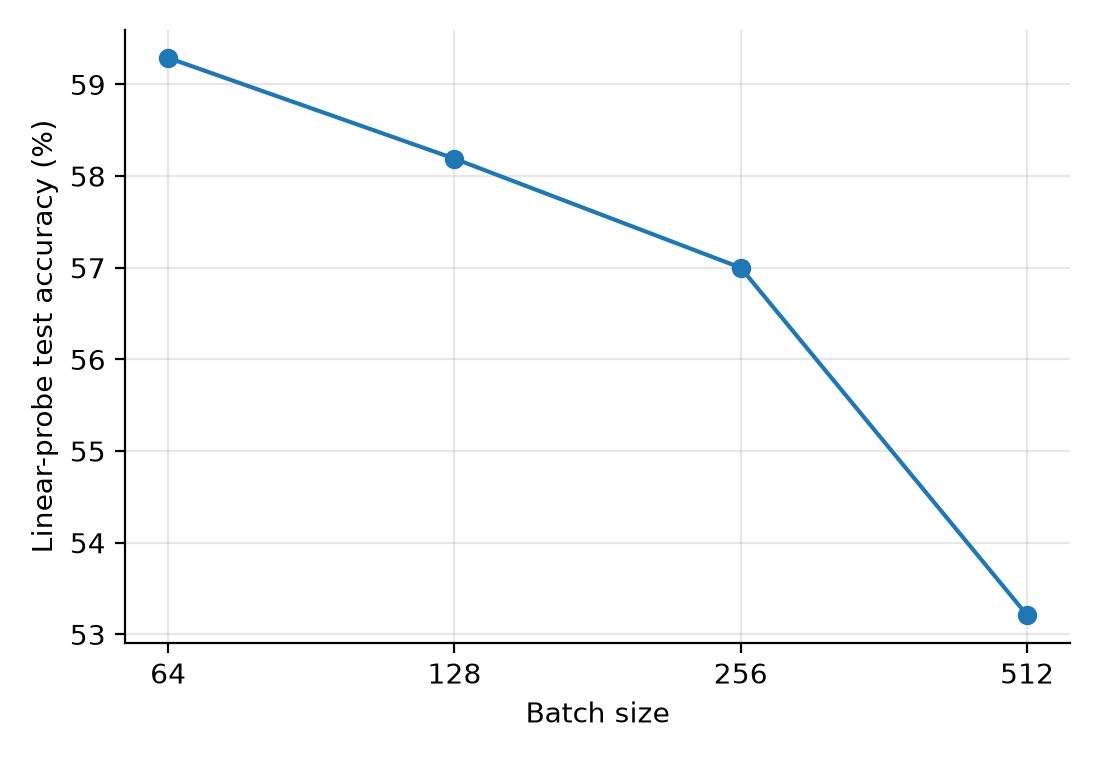
\includegraphics[width=0.85\linewidth]{../results/batchsize_ablation.png}
  \caption{Linear probe accuracy as a function of batch size (log$_2$ scale).}
  \label{fig:batchsize}
\end{figure}

\subsection{Analysis}

Table~\ref{tab:batchsize} shows that accuracy increases sharply from batch size 64
(49.09\%) to 128 (58.11\%), a gain of 9.02 percentage points. This is consistent with
the finding in Chen et al.\ \cite{chen2020simclr} that more negatives per image
strengthen the contrastive signal. Each image in a batch of size $B$ is contrasted
against $2B - 2$ other views during training; a larger denominator in the NT-Xent
softmax makes the task harder and forces the encoder to learn more discriminative
features.

Interestingly, accuracy \textit{decreases} beyond batch size 128: 56.35\% at 256 and
53.74\% at 512, both below the 128 peak. This non-monotonic behaviour is explained by
the interaction between batch size and the number of gradient updates under a fixed
compute budget. With 20 epochs and 20,000 images, batch size 128 gives
$\lfloor 20000/128 \rfloor \times 20 = 3{,}120$ update steps, while batch size 512
gives only $\lfloor 20000/512 \rfloor \times 20 = 760$ steps. The larger batch
provides more negatives per step but far fewer steps overall, and at this short
schedule the reduction in updates outweighs the benefit of additional negatives.
Linear learning rate scaling \cite{goyal2017scaling} would partly compensate, but
was not applied here since all runs used the same learning rate $3\times10^{-4}$.

Training time was broadly similar across all batch sizes (31--35 minutes on a T4),
because the total number of images processed per epoch is fixed by the subset size
rather than the batch size. GPU memory usage scales linearly with batch size, which
would become a hard constraint on hardware with less than 15,360\,MiB.

For this dataset and short schedule, batch size 128 gives the best linear probe
accuracy. Batch size 256 is a reasonable choice when longer training is available,
as the original SimCLR paper suggests the benefit of large batches materialises more
clearly with more training epochs.

% ================================================================
\section{Conclusion}
\label{sec:conclusion}

% [Shubham writes this section]
\textit{To be completed by Shubham.}

% ================================================================
\section*{Contributions}

\begin{itemize}
  \item \textbf{Shubham Kang:} SimCLR implementation, pretraining, augmentation
        ablation, analysis, abstract, method, discussion, conclusion, final PDF.
  \item \textbf{Sandhya Parmar:} Supervised baseline, linear probe and fine-tune
        evaluation, experimental setup section, results section.
  \item \textbf{Nidhi Kumari:} Batch-size ablation, figures, documentation,
        introduction, related work, batch-size analysis section, references.
\end{itemize}

% ================================================================
\begin{thebibliography}{99}

\bibitem{chen2020simclr}
T.\ Chen, S.\ Kornblith, M.\ Norouzi and G.\ Hinton,
``A simple framework for contrastive learning of visual representations,''
{\em Proceedings of the International Conference on Machine Learning (ICML)}, 2020.

\bibitem{coates2011stl10}
A.\ Coates, A.\ Ng and H.\ Lee,
``An analysis of single-layer networks in unsupervised feature learning,''
{\em Proceedings of the International Conference on Artificial Intelligence
and Statistics (AISTATS)}, 2011.

\bibitem{he2016resnet}
K.\ He, X.\ Zhang, S.\ Ren and J.\ Sun,
``Deep residual learning for image recognition,''
{\em Proceedings of the IEEE Conference on Computer Vision and Pattern
Recognition (CVPR)}, 2016.

\bibitem{krizhevsky2012imagenet}
A.\ Krizhevsky, I.\ Sutskever and G.E.\ Hinton,
``Imagenet classification with deep convolutional neural networks,''
{\em Advances in Neural Information Processing Systems (NeurIPS)}, 2012.

\bibitem{he2020moco}
K.\ He, H.\ Fan, Y.\ Wu, S.\ Xie and R.\ Girshick,
``Momentum contrast for unsupervised visual representation learning,''
{\em Proceedings of the IEEE Conference on Computer Vision and Pattern
Recognition (CVPR)}, 2020.

\bibitem{gidaris2018rotnet}
S.\ Gidaris, P.\ Singh and N.\ Komodakis,
``Unsupervised representation learning by predicting image rotations,''
{\em Proceedings of the International Conference on Learning
Representations (ICLR)}, 2018.

\bibitem{noroozi2016jigsaw}
M.\ Noroozi and P.\ Favaro,
``Unsupervised learning of visual representations by solving jigsaw puzzles,''
{\em Proceedings of the European Conference on Computer Vision (ECCV)}, 2016.

\bibitem{zhang2016colorization}
R.\ Zhang, P.\ Isola and A.A.\ Efros,
``Colorful image colorization,''
{\em Proceedings of the European Conference on Computer Vision (ECCV)}, 2016.

\bibitem{wu2018unsupervised}
Z.\ Wu, Y.\ Xiong, S.\ Yu and D.\ Lin,
``Unsupervised feature learning via non-parametric instance discrimination,''
{\em Proceedings of the IEEE Conference on Computer Vision and Pattern
Recognition (CVPR)}, 2018.

\bibitem{goyal2017scaling}
P.\ Goyal, P.\ Doll{\'a}r, R.\ Girshick, P.\ Noordhuis, L.\ Wesolowski,
A.\ Kyrola, A.\ Tulloch, Y.\ Jia and K.\ He,
``Accurate, large minibatch {SGD}: Training {ImageNet} in 1 hour,''
{\em arXiv preprint arXiv:1706.02677}, 2017.

\end{thebibliography}

\end{document}
